%! TEX root = **/010-main.tex
% vim: spell spelllang=en:

%%%%%%%%%%%%%%%%%%%%%%%%%%%%%%%%%%%%%%%%%%%%%%%%%%%%%%%%%%%%%%%%%%%%%%%%%%%%%%%%
% PREAMBLE
%%%%%%%%%%%%%%%%%%%%%%%%%%%%%%%%%%%%%%%%%%%%%%%%%%%%%%%%%%%%%%%%%%%%%%%%%%%%%%%%
%! TEX root = **/010-main.tex
%%%%%%%%%%%%%%%%%%%%%%%%%%%%%%%%%%%%%%%%%%%%%%%%%%%%%%%%%%%%%%%%%%%%%%%%%%%%%%%%
%% LaTeX preamble, load in main.tex with: \input{preamble}
%%%%%%%%%%%%%%%%%%%%%%%%%%%%%%%%%%%%%%%%%%%%%%%%%%%%%%%%%%%%%%%%%%%%%%%%%%%%%%%%

\documentclass[12pt, oneside, final]{article}
% \usepackage[a4paper, left=2.5cm, right=2.5cm, top=2.5cm, bottom=2.5cm]{geometry}
\usepackage[a4paper]{geometry}
% \usepackage[a4paper,showframe]{geometry}

\setlength{\headheight}{24pt}

% for debugging overfulls
%\documentclass[draft, 12pt, oneside]{article}
%\usepackage[showframe, a4paper, left=2.5cm, right=2.5cm, top=2.5cm, bottom=2.5cm]{geometry}

%%%%%%%%%%%%%%%%%%%%%%%%%%%%%%%%%%%%%%%%%%%%%%%%%%%%%%%%%%%%%%%%%%%%%%%%%%%%%%%%
%% FONTS
%%%%%%%%%%%%%%%%%%%%%%%%%%%%%%%%%%%%%%%%%%%%%%%%%%%%%%%%%%%%%%%%%%%%%%%%%%%%%%%%

\usepackage[T1]{fontenc}
\usepackage{fontspec}
\usepackage{microtype}

\setmonofont[Scale=MatchLowercase]{DejaVu Sans Mono}

%%%%%%%%%%%%%%%%%%%%%%%%%%%%%%%%%%%%%%%%%%%%%%%%%%%%%%%%%%%%%%%%%%%%%%%%%%%%%%%%
%% LANGUAGE
%%%%%%%%%%%%%%%%%%%%%%%%%%%%%%%%%%%%%%%%%%%%%%%%%%%%%%%%%%%%%%%%%%%%%%%%%%%%%%%%

\usepackage{polyglossia}
\setdefaultlanguage{english}
\setotherlanguages{spanish,catalan}

%%%%%%%%%%%%%%%%%%%%%%%%%%%%%%%%%%%%%%%%%%%%%%%%%%%%%%%%%%%%%%%%%%%%%%%%%%%%%%%%
%% BIBLIOGRAPHY
%%%%%%%%%%%%%%%%%%%%%%%%%%%%%%%%%%%%%%%%%%%%%%%%%%%%%%%%%%%%%%%%%%%%%%%%%%%%%%%%

\usepackage[
    backend=biber,
    style=numeric,
]{biblatex}
\DeclareNameAlias{default}{family-given}

\addbibresource{biblio.bib}

\usepackage{fvextra}        % Req by minted (must load before csquotes)
\usepackage{csquotes}       % For bibliography quotations
\DeclareQuoteAlias{spanish}{catalan}

%%%%%%%%%%%%%%%%%%%%%%%%%%%%%%%%%%%%%%%%%%%%%%%%%%%%%%%%%%%%%%%%%%%%%%%%%%%%%%%%
%% COMMON
%%%%%%%%%%%%%%%%%%%%%%%%%%%%%%%%%%%%%%%%%%%%%%%%%%%%%%%%%%%%%%%%%%%%%%%%%%%%%%%%

\usepackage{color, xcolor}     % more colors

\usepackage{graphicx}   % graphics
\graphicspath{{./figures/}}

\usepackage{comment}

%%%%%%%%%%%%%%%%%%%%%%%%%%%%%%%%%%%%%%%%%%%%%%%%%%%%%%%%%%%%%%%%%%%%%%%%%%%%%%%%
%% MATHS
%%%%%%%%%%%%%%%%%%%%%%%%%%%%%%%%%%%%%%%%%%%%%%%%%%%%%%%%%%%%%%%%%%%%%%%%%%%%%%%%

\usepackage{mathtools}  % amsmath + more
\usepackage{amsthm}     % Theorem enviroment
\usepackage{amssymb}    % More symbols
\usepackage{amstext}    % Text inside mathenv

%\usepackage{relsize}    % Bigger math with mathlarger{___}
\usepackage{nicefrac}   % nice fractions in one line

%\usepackage{IEEEtrantools} % Complex equation arrays

%%%%%%%%%%%%%%%%%%%%%%%%%%%%%%%%%%%%%%%%%%%%%%%%%%%%%%%%%%%%%%%%%%%%%%%%%%%%%%%%
%% REFERENCES (load order is important)
%%%%%%%%%%%%%%%%%%%%%%%%%%%%%%%%%%%%%%%%%%%%%%%%%%%%%%%%%%%%%%%%%%%%%%%%%%%%%%%%

\usepackage{varioref} % reference far away (1)
\usepackage[colorlinks = true]{hyperref} % links in references (2)
\usepackage{cleveref} % smart references (3)
%hyperref configuration so that it doesn't contrast so much colorlinks,
\hypersetup{
   linkcolor={black},
   citecolor={black},
   %linkcolor={red!50!black},
   %citecolor={blue!50!black},
   urlcolor={blue!80!black}
}

\usepackage[bottom]{footmisc} % Footnotes at bottom of page

%%%%%%%%%%%%%%%%%%%%%%%%%%%%%%%%%%%%%%%%%%%%%%%%%%%%%%%%%%%%%%%%%%%%%%%%%%%%%%%%
%% FIGURES
%%%%%%%%%%%%%%%%%%%%%%%%%%%%%%%%%%%%%%%%%%%%%%%%%%%%%%%%%%%%%%%%%%%%%%%%%%%%%%%%

%\usepackage[export]{adjustbox}  % Adjust table size
\usepackage{float}               % Force tables and images position (H and H!)
%\usepackage{wrapfig}            % Wrap images like in HTML

\usepackage[justification=centering]{caption}
%\usepackage{subcaption}                     % Subfigures
%\usepackage[framemethod=tikz]{mdframed}     % Custom frames

%%%%%%%%%%%%%%%%%%%%%%%%%%%%%%%%%%%%%%%%%%%%%%%%%%%%%%%%%%%%%%%%%%%%%%%%%%%%%%%%
%% TABLES
%%%%%%%%%%%%%%%%%%%%%%%%%%%%%%%%%%%%%%%%%%%%%%%%%%%%%%%%%%%%%%%%%%%%%%%%%%%%%%%%

%\usepackage{colortbl, booktabs} % Better tables
%\usepackage{tabularx}
%\usepackage{longtable} % Multiple page table (does not work with tabularx)
\usepackage{xltabular, colortbl, booktabs} % longtable + tabularx (has bug with booktabs: fix below)

% Split cell in lines and more formating options inside table
\usepackage{array, multirow, multicol, makecell}

%%%
% bug fix for booktabs + xltabular incompatibility
\makeatletter
\def\@BTrule[#1]{%
  \ifx\longtable\undefined
    \let\@BTswitch\@BTnormal
  \else\ifx\hline\LT@hline
    \nobreak
    \let\@BTswitch\@BLTrule
  \else
     \let\@BTswitch\@BTnormal
  \fi\fi
  \global\@thisrulewidth=#1\relax
  \ifnum\@thisruleclass=\tw@\vskip\@aboverulesep\else
  \ifnum\@lastruleclass=\z@\vskip\@aboverulesep\else
  \ifnum\@lastruleclass=\@ne\vskip\doublerulesep\fi\fi\fi
  \@BTswitch}
\makeatother
%%%

%%%%%%%%%%%%%%%%%%%%%%%%%%%%%%%%%%%%%%%%%%%%%%%%%%%%%%%%%%%%%%%%%%%%%%%%%%%%%%%%
%% SIUNITX
%%%%%%%%%%%%%%%%%%%%%%%%%%%%%%%%%%%%%%%%%%%%%%%%%%%%%%%%%%%%%%%%%%%%%%%%%%%%%%%%

\usepackage{siunitx}                        % SI units and uncertainties
%\sisetup{locale = FR}                       % Commas and so on for spanish
%\sisetup{separate-uncertainty=true}
\sisetup{
  per-mode=fraction,
  fraction-function=\nicefrac
}

%%%%%%%%%%%%%%%%%%%%%%%%%%%%%%%%%%%%%%%%%%%%%%%%%%%%%%%%%%%%%%%%%%%%%%%%%%%%%%%%
%% TIKZ
%%%%%%%%%%%%%%%%%%%%%%%%%%%%%%%%%%%%%%%%%%%%%%%%%%%%%%%%%%%%%%%%%%%%%%%%%%%%%%%%

%\usepackage{tikz}
%\usetikzlibrary{arrows}
%\usetikzlibrary{scopes}
%\usetikzlibrary{babel}

%%%%%%%%%%%%%%%%%%%%%%%%%%%%%%%%%%%%%%%%%%%%%%%%%%%%%%%%%%%%%%%%%%%%%%%%%%%%%%%%
%% MINTED
%%%%%%%%%%%%%%%%%%%%%%%%%%%%%%%%%%%%%%%%%%%%%%%%%%%%%%%%%%%%%%%%%%%%%%%%%%%%%%%%

\usepackage{minted}
\definecolor{codeBg}{HTML}{FFFDE7}
\setminted{
    %style=pastie,
    frame=lines,
    framesep=3mm,
    linenos,
    breaklines=true,
    encoding=utf8,
    fontsize=\footnotesize,
    bgcolor=codeBg
}

%%%%%%%%%%%%%%%%%%%%%%%%%%%%%%%%%%%%%%%%%%%%%%%%%%%%%%%%%%%%%%%%%%%%%%%%%%%%%%%%
%% CUSTOM COMMANDS
%%%%%%%%%%%%%%%%%%%%%%%%%%%%%%%%%%%%%%%%%%%%%%%%%%%%%%%%%%%%%%%%%%%%%%%%%%%%%%%%

% empty whitepage without numbering
\newcommand{\whitepage}{
    \clearpage\thispagestyle{empty}\addtocounter{page}{-1} \newpage \clearpage
}

% Add command before appendix section for page numbering: A-1
\newcommand{\appendixpagenumbering}{
    \break
    \pagenumbering{arabic}
    \renewcommand{\thepage}{\thesection-\arabic{page}}
}

%%%%%%%%%%%%%%%%%%%%%%%%%%%%%%%%%%%%%%%%%%%%%%%%%%%%%%%%%%%%%%%%%%%%%%%%%%%%%%%%
%% CUSTOM MATH OPERATORS (functions not in italic in math mode)
%%%%%%%%%%%%%%%%%%%%%%%%%%%%%%%%%%%%%%%%%%%%%%%%%%%%%%%%%%%%%%%%%%%%%%%%%%%%%%%%

%\DeclareMathOperator{\arcsec}{arcsec}
%\DeclareMathOperator{\arccot}{arccot}
%\DeclareMathOperator{\arccsc}{arccsc}
%\DeclareMathOperator{\cis}{cis}

%%%%%%%%%%%%%%%%%%%%%%%%%%%%%%%%%%%%%%%%%%%%%%%%%%%%%%%%%%%%%%%%%%%%%%%%%%%%%%%%
%% MISC
%%%%%%%%%%%%%%%%%%%%%%%%%%%%%%%%%%%%%%%%%%%%%%%%%%%%%%%%%%%%%%%%%%%%%%%%%%%%%%%%

%\usepackage{datetime} % Customize date
%% \monthyeardate\today gives the date without the day
%\newdateformat{monthyeardate}{%
    %\monthname[\THEMONTH], \THEYEAR}


%%%%%%%%%%%%%%%%%%%%%%%%%%%%%%%%%%%%%%%%%%%%%%%%%%%%%%%%%%%%%%%%%%%%%%%%%%%%%%%%
% EXTRA PACKAGES / CONFIG
%%%%%%%%%%%%%%%%%%%%%%%%%%%%%%%%%%%%%%%%%%%%%%%%%%%%%%%%%%%%%%%%%%%%%%%%%%%%%%%%

\usepackage{fancyhdr}
\usepackage{pgfgantt}
\usepackage{pdflscape}
\usepackage{titlesec}

\usepackage{chngcntr}
\counterwithin{figure}{section}
\counterwithin{table}{section}

% paragraph in newline
\titleformat{\paragraph}[hang]{\normalfont\normalsize\bfseries}{\theparagraph}{1em}{}
\titlespacing*{\paragraph}{0pt}{3.25ex plus 1ex minus .2ex}{0.5em}

% bold \thead (table headers)
\renewcommand\theadfont{\bfseries}

%%%%%%%%%%%%%%%%%%%%%%%%%%%%%%%%%%%%%%%%%%%%%%%%%%%%%%%%%%%%%%%%%%%%%%%%%%%%%%%%
% METADATA
%%%%%%%%%%%%%%%%%%%%%%%%%%%%%%%%%%%%%%%%%%%%%%%%%%%%%%%%%%%%%%%%%%%%%%%%%%%%%%%%
\title{High-performance simulation of the 16th Hilbert's problem}
\author{Aleix Bon\'e Rib\'o}
\date{\today}

\begin{document}
%%%%%%%%%%%%%%%%%%%%%%%%%%%%%%%%%%%%%%%%%%%%%%%%%%%%%%%%%%%%%%%%%%%%%%%%%%%%%%%%
% TITLE
%%%%%%%%%%%%%%%%%%%%%%%%%%%%%%%%%%%%%%%%%%%%%%%%%%%%%%%%%%%%%%%%%%%%%%%%%%%%%%%%

    % Default title or use titlepage.tex

    %\maketitle
    %! TEX root = **/010-main.tex
% vim: spell spelllang=en:

\thispagestyle{empty}
\clearpage
\setcounter{page}{-1}

\makeatletter
\begin{titlepage}
{
    \centering
    
\includegraphics[width=0.9\textwidth]{logo-upc}
    \null
    \vspace{3em}
    {\Huge \bfseries \@title \par}
    \vspace{2em}
    {\large Project management (GEP) \\
        (Budget and sustainability) %todo change
    \par}
    \vspace{3em}
    {\large \scshape \@date \par}

    \vfill
    {\raggedleft \large \bfseries \@author \par}
    \vspace{1em}
    {\raggedleft \large
        Bachelor thesis \\
        Specialization in Computing \\
        \vspace{2em}
        Director: Grigori Astrakharchik \\
        GEP Tutor: Eguiguren Huerta Marcos
    \par}
}
\end{titlepage}
\makeatother


%%%%%%%%%%%%%%%%%%%%%%%%%%%%%%%%%%%%%%%%%%%%%%%%%%%%%%%%%%%%%%%%%%%%%%%%%%%%%%%%
% TOC & lists
%%%%%%%%%%%%%%%%%%%%%%%%%%%%%%%%%%%%%%%%%%%%%%%%%%%%%%%%%%%%%%%%%%%%%%%%%%%%%%%%

    \pagenumbering{Roman}

    %\setcounter{tocdepth}{2}
    \tableofcontents% \pagebreak

    \listoffigures %\pagebreak
    \listoftables \clearpage

    \pagenumbering{arabic}

%%%%%%%%%%%%%%%%%%%%%%%%%%%%%%%%%%%%%%%%%%%%%%%%%%%%%%%%%%%%%%%%%%%%%%%%%%%%%%%%
% SECTIONS
%%%%%%%%%%%%%%%%%%%%%%%%%%%%%%%%%%%%%%%%%%%%%%%%%%%%%%%%%%%%%%%%%%%%%%%%%%%%%%%%

    % Paragraph spacing (placed after ToC)
    \setlength{\parskip}{1em plus 0.5em minus 0.2em}
    %\setlength{\parindent}{0pt}

    \pagestyle{fancy}
    \fancyhf{}

    \makeatletter
        \fancyhead[L]{\@title}
        \fancyfoot[L]{Chapter \thesection}
        \fancyfoot[C]{\@author}
        \fancyfoot[R]{\thepage}
    \makeatother

    \renewcommand{\headrulewidth}{1pt}
    \renewcommand{\footrulewidth}{0.75pt}

    % GEP
    %! TEX root = **/010-main.tex
% vim: spell spelllang=en:

\section{Context and scope}%
\label{sec:context}

\subsection{Introduction and contextualization}%
\label{sub:intro}

Since its release in 2007, Compute Unified Device Architecture (CUDA) has
revolutionized the usage of graphic processing units for scientific
computations, allowing developers to implement programs that take full advantage
of the parallelization capabilities of GPUs for general purpose programming.
This paired with the exponential growth of computing power that GPUs have
experienced in the last decade has made GPU numerical analysis essential on
modern science research. Highly complex problems that where once impossible to
compute in realistic time frames can now be computed even on average consumer
hardware GPUs. Moreover, projects like
\emph{GPUGRID}\footnote{\url{www.gpugrid.net}} allow researches to run
distributed programs through a grid of GPUs from volunteers all over the world
reaching supercomputing level performance \cite{antaviana_nvidia_nodate}.


In 1900 David Hilbert posed a list of 23 problems in the field of mathematics
which were unsolved at the time \cite{hilbert_mathematische_1900}.  Those
problems have been vastly studied since then and most of them are solved or
partially solved. There are however some which are still unsolved to this day.

One of these unsolved problems is the 16th problem.  This problem consists of
two separate problems, the first one regarding the relative positions of the
branches of real algebraic curves and the second one about the upper limit of
limit cycles on two dimensional vector fields and their relative positions. In
this project we are going to study the second part of this 16th problem.

In particular, we study the number of limit cycles for vector fields of
polynomials of second degree:
\begin{align}\label{eq:system}
    \frac{dx}{dt} &= a_1x^2 + b_1xy + c_1y^2 + \alpha_1x + \beta_1y \nonumber \\
    \frac{dy}{dt} &= a_2x^2 + b_2xy + c_2y^2 + \alpha_2x + \beta_2y
\end{align}


\pagebreak
It is unknown whether there exists an upper limit on the number of limit cycles
for systems with polynomials of degree greater than
one\cite{ilyashenko_centennial_2002,llibre_16hilbert_nodate}.  Nowadays, the
largest number of limit cycles found is equal to four and it is still an open
question whether or not a larger number of limit cycles is possible. Therefore,
finding a system with more than 4 limit cycles will be quite an important result
for the academic community.

To find interesting systems several combinations of the equation parameters
must be tried and evaluated, since each of this systems can be computed
independently from the rest they can all be run in parallel, making it an ideal
problem to compute in massively parallel GPU nodes.

\subsubsection{Context}

This is a Bachelor Thesis of the Computer Engineering Degree, specialization in
Computing, done in the Facultat Inform\`atica de Barcelona (FIB) of the
Universitat Polit\'ecnica de Catalunya (UPC). The project is directed by Grigori
Astrakharchik.

\subsubsection{Concepts}

Below are some concepts needed to understand the project.

\newcommand{\concept}[1]{\textbf{#1}\\}

\concept{Limit cycles}
A limit cycle is a closed trajectory with the property that at least one other
trajectory spirals into it as time approaches infinity. They are important in
various applications in the field of dynamical systems.

\concept{CUDA}
CUDA is a parallel computing platform developed by \emph{nvidia} that allows general
computing on their graphic processing units (GPUs). Using the CUDA programming
model allows developers to run massively parallel programs on GPUs.

\pagebreak
\subsubsection{Problem to be solved}

There have been various studies on the number of limit cycles for second degree
vector fields but so far the maximum number of cycles found is 4, as shown in
Ref.~\cite{kuznetsov_visualization_2013}. The aim of this project is to search
the parameter space for systems that have 4 or more cycles to gain more insight
on the nature of these equations.

\Cref{fig:kuznetsov} shows a characteristic example of a visualization of the
limit cycles in a two-dimensional polynomial quadratic system.

\begin{figure}[H]
    \centering
    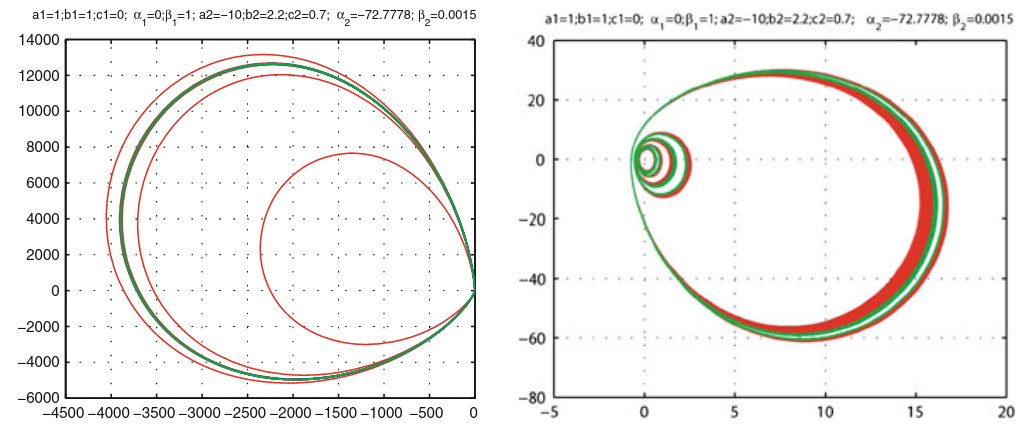
\includegraphics[width=1.0\textwidth]{4cycles}
    \caption{Visualization of four limit cycles in two-dimensional polynomial quadratic system, from Ref.~\cite{kuznetsov_visualization_2013}
    }%
    \label{fig:kuznetsov}
\end{figure}

To do so, we will implement an efficient parallel algorithm that solves systems
of ordinary differential equations (ODE) and detects limit cycles for a wide
range of parameters and points in the plane.  This code will be implemented in
Julia programming language and will use CUDA framework in such a way that
massive parallel calculation can be done on a dedicated CUDA server with several
advanced GPU graphic cards.

\pagebreak

\subsection{Computational complexity}

In~\cref{eq:system} we have 5 parameters for $x$ and 5 for $y$ which makes a
total of 10 distinct parameters. Adding the initial point to calculate the
trajectories ($x$ and $y$ coordinates) it makes a total of 12 parameters.
However we will only consider the reduced for of the system which only has 5
parameters (parameters for $x$ are 1) as shown in~\cref{eq:system2}. This gives
a total of 7 parameters.

\begin{align}\label{eq:system2}
    \frac{dx}{dt} &= x^2 + xy + y^2 + x + y \nonumber \\
    \frac{dy}{dt} &= a_2x^2 + b_2xy + c_2y^2 + \alpha_2x + \beta_2y
\end{align}


If we consider $n$ different values for each of those parameters we have a total
of $n^7$ different trajectories to calculate. If we were to compute the
trajectories sequentially it would take a long time for moderately sized values
of $n$. Calculating a trajectory on my machine takes 0.01 seconds. This means
that for $n=10$ it would take approximately 28 hours to compute all the
trajectories and taking $n=30$ the time increases to 7 years. If we use a GPU
with 5000 CUDA cores (Tesla K90) it would only take 20 seconds (assuming perfect
parallelization which is unrealistic). And for $n=30$ it would take 12 and a
half hours. If we consider the usage of a super computer like the Mare nostrum
with a cluster of 39 servers with 2 Tesla K90 GPUs the time for $n=30$ is a mere
9 minutes. \footnote{All these calculations are based on a very rough estimate
of the computing time needed to determine the limit cycle of a trajectory which
may vary a lot depending on the system and the implementation of the code}

\subsubsection{Stakeholders}

The main stakeholder in this project is the director Grigori Astrakharchik who
has a direct implication on the Thesis.

\pagebreak
\subsection{Justification}
\subsubsection{Previous studies}

In~\cite{kuznetsov_visualization_2013} there is a description of a task given by
the academician A.N. Kolmogorov:

\begin{quote}
To estimate the number of limit cycles of square vector fields on plane, A.N. Kolmogorov had
distributed several hundreds of such fields (with randomly chosen coefficients
of quadratic expressions) among a few hundreds of students of Mech \& Math
Faculty of Moscow State University as a mathematical practice. Each student had
to find the number of limit cycles of a field. The result of this experiment was
absolutely unexpected: not a single field had a limit cycle!
\end{quote}

This shows that the parallelizable nature of the problem and how difficult it is
to find those cycles. Therefore it is important to implement a code that is both
efficient on the calculation and have a big enough search space to find results.

There have been a number of studies relying on numerical methods to find limit
cycles in two dimensional vector fields
\cite{leonov_hidden_2013,van_der_hoff_numerical_2013,casades_computation_2013,gasull_effective_nodate}.
Papadimitriou and Vishnoi showed that the computation of a limit cycle is
% todo
% PSPACE??
\textbf{PSPACE}-complete~\cite{papadimitriou_computational_2015}.
The maximal known number of limit cycles is reported in Kuznetsov et
al.~\cite{kuznetsov_visualization_2013} where an example of specific conditions
for which 4 limit cycles is provided.

% todo

The CUDA framework has API for several programming languages (C, C++, Fortran,
Python, MATLAB, \dots). The official programming toolkit is in C/C++ and offers
the most customizability and low level configuration to adapt the code to the
hardware. The two most notable alternatives are Python's pyCUDA and Julia's
CUDA.jl libraries. These libraries bind to the C CUDA API and interface the data
between the kernels and the programming language. As such, the performance of
the kernels that run in the GPU should be equivalent in all cases but the data
models and processing of different languages makes a difference when interfacing
between the GPU code and the CPU code.

However, languages such as Python and Julia allow for faster coding and easier
visualization of the data. For this Thesis we will use Julia programming
language since it's faster than Python, has many libraries and tools for
numerical analysis and has type checking.  Nonetheless, this is not a strict
constraint and the possibility of writing specific C CUDA code to tweak the
performance to the maximum will be studied.

% There are various programming languages (C, C++, Fortran, Python and MATLAB) compatible with CUDA and which have libraries for CUDA programming.
%There are various programming languages with libraries for CUDA programming.
%In GPU-accelerated applications, the sequential part of the workload runs on the CPU – which is optimized for single-threaded performance – while the compute intensive portion of the application runs on thousands of GPU cores in parallel. When using CUDA, developers program in popular languages such as C, C++, Fortran, Python and MATLAB and express parallelism through extensions in the form of a few basic keywords.
%The official CUDA programming model is in C/C++ and offers the most flexibility and performance. The other two most notable alternatives are Python's Numba and Julia's CUDA.jl.
%These are higher-level libraries and
%are more limited in the versatility
%%do not offer the same low level options
%but allow easier development and visualization of the data.
%Both Python and Julia use the official CUDA C interface under the hood so
%although the performance is not as good as with pure C, if an appropriate
%realization of the methods is done, the performance might be still good if the
%majority of the work is done in the CUDA kernels. Since Julia JIT compilation is
%faster than the python's one and provides similar advantages when visualizing
%data the initial idea is to program the whole project in Julia programming
%language.


% todo

\pagebreak
\subsection{Scope}
\subsubsection{Objectives and sub-objectives}

The main objective of this Thesis is to develop a highly-efficient code capable
of determining the possible existence of limit cycles for a system. This code
must also be capable of being executed in parallel in a GPU cluster making full
use of its computing power to simulate a wide variety of systems with different
parameters. Furthermore, the results must be processed to find interesting
systems to visualize and analyse in more detail. These objectives can be divided
in sub-objectives:

\paragraph{Theoretical part}

Before implementing the algorithms and developing the code, a deep understanding
of the current numerical methods and the CUDA framework must be achieved to find
the best approach to the problem.

\begin{itemize}
    \item Explore the best strategies to solve ordinary differential equations.
    \item Explore numerical methods to verify the existence of limit cycles and determine the number of cycles for a given system.
    \item Research how these methods can be applied to run in a CUDA system efficiently.
\end{itemize}

\paragraph{Practical part} Having done the background research, the code must be
developed, implemented and tested.  Different methods will be tried in order to
find the ones that give the best performance.

\begin{itemize}
    \item Implement the algorithms in an efficient code.
    \item Benchmark the performance and compare different approaches to achieve the best performance.
    \item Run the code on a dedicated GPU server.
    \item Analyse the results and visualize them.
    \item Present and discuss the obtained results in the Thesis.
\end{itemize}

\subsubsection{Requirements}

To ensure the quality of the Thesis a number of requirements must be fulfilled:
\begin{itemize}
    \item Find the best balance between accuracy of the results and computational complexity
    \item Ensure that the numerical methods applied are properly implemented.
    \item Take into account numerical stability of the methods used as well as rounding and overflow errors.
    \item Profile the different methods under the same conditions and environment to ensure that there are no biases.
    \item Use good programming practices, making readable and maintainable code with the least complexity possible.
    \item Make the developed code publicly available.
\end{itemize}

\subsubsection{Potential obstacles and risks}

There are several risks that may have to be dealt with during the development of this Thesis.

\begin{itemize}
    \item \textbf{Project deadlines}: There is a limited amount of time to do
        the project. Therefore, a proper planning of tasks and time must be made
        and followed to ensure that the work can be done in the proper time
        frame.
    \item \textbf{Computational power}: This Thesis involves a lot of
        computational power and the whole project is conditioned by it. If the
        program cannot be run on the proper hardware the results may not be
        obtainable in a realistic time frame and the scope of the project will
        have to be reevaluated.
    \item \textbf{Inexperience on the field}: I have very limited experience
        with CUDA programming and just the basics of numerical computation
        techniques so there is a lot of research to be done, specially regarding
        dynamical systems.
\end{itemize}

\pagebreak
\subsection{Methodology and rigor}

\subsubsection{Methodology}

Since the Thesis must be completed in a relatively short period of time we will
apply the \emph{agile} methodology and divide the work into sub-tasks or
\emph{sprints}. These \emph{sprints} will consist of different stages of
implementation of the program, beginning with a proof of concept running in
sequence on the CPU and progressively iterating on this base to optimize the
methods and adapt them to be able to run in CUDA on the GPU.

\subsubsection{Monitoring tools and validation}

To manage the different iterations of the code \texttt{git} will be used. The
repository will be hosted on \emph{GitHub} and access will be granted to the
project tutor allowing him to follow and monitor the work and results at any
time.

A weekly meeting with the tutor will be arranged to discuss the progress and
which tasks should be worked on.

    %! TEX root = **/010-main.tex
% vim: spell spelllang=en:

\section{Time planning}

The work-to-begin date is on February 9th and the delivery date on June which
gives around 18 weeks of time. I plan to work on the project approximately 35
hours a week, this gives around 630 hours in total working on the project.

\subsection{Description of the tasks}

\subsubsection{Task definition}

The definitions of the tasks that will be done throughout the project are
divided into 4 categories: planning, research, implementation and experimentation.

\paragraph{Project planning}

\begin{itemize}
    \item \textbf{Contextualization and project scope} Describe the project
        scope and its context. Giving an overview of the objective, other past
        studies on the topic and how this project is relevant.
    \item \textbf{Time planning} Organize the work to be done in granular tasks
        to estimate the time needed for each of them. With the time estimation
        create a realistic planning for the tasks completions so that the
        project can be finished in the appropriate time frame.
    \item \textbf{Budget and sustainability} Analyze the economic and
        environmental sustainability of the project.
    \item \textbf{Meetings} Each week a meeting with the tutor will be scheduled
        to ensure that the thesis is proceeding correctly and within the
        expected deadlines.
    \item \textbf{Integration into the final document} All these project
        planning tasks must be integrated into the final thesis memoir.
\end{itemize}

\paragraph{Research}

Given the nature of this thesis it is fundamental to have a solid understanding
of modern numerical computation techniques applied to solving Ordinary
Differential Equations and finding limit cycles. It is also primordial to know
how these techniques can be applied to CUDA and how to benchmark the programs to
detect bottlenecks and find whether or not the processing power of the GPU is
being used in its full potential.

\begin{itemize}
    \item \textbf{Research ODE solvers} There are lots of algorithm to solve
        ODEs which will have to be tried to find the ones that give the best
        results in our case.
    \item \textbf{Research how to find limit cycles} Find the best approach to
        detect limit cycles
    \item \textbf{Research CUDA} This task includes reading the official
        documentation as well as other sources on numerical methods applied to
        CUDA.
\end{itemize}

\paragraph{Practical Implementation}

The different algorithms researched must be implemented in order to experiment
with them and find the best ones to solve the problem.

\begin{itemize}
    \item \textbf{Program different methods to find limit cycles} As stated
        before various different methods will have to be implemented. This
        implementation can be initially without using CUDA (fully sequential).
    \item \textbf{Adapt de code to be run with CUDA} Once the methods to find
        limit cycles are properly implemented they must be adapted in order to
        be run with CUDA.
    \item \textbf{Test the program} In order to ensure that the code implemented
        is correct and the errors introduced in the computation fall within a
        reasonable distance of the real theoretical value some tests must be
        implemented. This includes also the implementation of small programs to
        visualize the results and interpret them.
\end{itemize}

\paragraph{Experimentation, analysis and conclusions}

Once there is a working prototype of the code the experimentation can begin.
There will be two major parts of the experimentation, the first one when the
various methods are tested with a relatively small number of cases to find the
best one (taking into account both the speed and accuracy of the calculations)
and the final experiment when the best method is run with a much bigger search
space and from which the results can be analysed.

\begin{itemize}
    \item \textbf{Comparison experiment}
        \begin{itemize}
            \item \textbf{Select search space} Decide how many different
                parameters will be used on the experiment. It should be a big
                enough search space so as to have variety on the systems but not
                big enough that it takes too much time to benchmark and slows
                down the development.
            \item \textbf{Select benchmarks} The benchmarks must be run in
                similar conditions and we must decide what metrics will be
                considered (runtime, GFLOPS, accuracy, \dots).
            \item \textbf{Further optimize the methods} When running the
                benchmarks we may find some possible improvements on the
                original implementations which can then be improved and tested
                again.
            \item \textbf{Analyse results and decide best method} With the
                results of the experiments we can decide on which method is the
                best and should therefore be used in the final experiment.
        \end{itemize}
    \item \textbf{Final experiment}
        \begin{itemize}
            \item \textbf{Select search space} Given the results of the previous
                experiments, estimate the runtime as a function of the search
                space and select a search space as big as possible given the
                available computing time.
            \item \textbf{Analyse results} Once the final experiment finishes
                the results can be analysed in search of systems with
                interesting number of limit cycles.
        \end{itemize}
    \item \textbf{Conclusions} Analyse the results of both experiments and
        provide a conclusion.
\end{itemize}

\pagebreak
\subsubsection{Summary of the tasks}

\begin{table}[H]
    \centering
    \caption{Summary of tasks}
    \begin{tabular}{llrc}
        \toprule
        \thead{ID} & \thead[l]{Task} & \thead{Time (h)} & \thead{Depend.} \\
        \midrule
    \texttt{P} & \textbf{Project planning} & \textbf{60} & \\
        \texttt{P0} & - Contextualization and project scope & 10 & \\
        \texttt{P1} & - Time planning & 10 & \\
        \texttt{P2} & - Budget and sustainability & 10 & \\
        \texttt{P3} & - Meetings & 18 & \\
        \texttt{P4} & - Integration into final document & 12 & \\

        \addlinespace[0.5em]
    \texttt{R} & \textbf{Research} & \textbf{150} & \\
        \texttt{R0} & - ODE solvers & 50 & \\
        \texttt{R1} & - Limit cycles & 50 & \\
        \texttt{R2} & - CUDA & 50 & \\

        \addlinespace[0.5em]
    \texttt{I} & \textbf{Implementation} & \textbf{200} & \\
        \texttt{I0} & - Different methods to find limit cycles & 100 & \texttt{R0,R1} \\
        \texttt{I1} & - Adapt to CUDA & 50 & \texttt{I0,R2} \\
        \texttt{I2} & - Tests & 50 & \\

        \addlinespace[0.5em]
    \texttt{EC} & \textbf{Experimentation (comparison)} & \textbf{130} & \texttt{I} \\
        \texttt{EC0} & Select search space & 5 & \\
        \texttt{EC1} & Select benchmarks & 5 & \\
        \texttt{EC2} & Further optimize the methods & 100 & \\
        \texttt{EC3} & Analyse the results and decide the best method & 20 & \\

    \addlinespace[0.5em]
    \texttt{EF} & \textbf{Experimentation (final)} & \textbf{25} & \texttt{EC} \\
        \texttt{EF0} & Select search space & 5 & \\
        \texttt{EF1} & Analyse the results & 20 & \\

    \addlinespace[0.5em]
        \texttt{C} & \textbf{Conclusions} & \textbf{10} & \texttt{EC,EF} \\
        \texttt{D} & \textbf{Documentation} & \textbf{60} & \\
        \texttt{O} & \textbf{Oral exposition} & \textbf{10} & \\
        \bottomrule
    \end{tabular}
\end{table}
% table

\pagebreak
\subsubsection{Resources}

\paragraph{Human resources}

The main human resource of the thesis is the researcher.  There is also the
director Grigori Astrakharchik which mentors the researcher and the GEP Tutor
Eguiguren Huerta Marcos in charge of correcting the project management part.

\paragraph{Material resources}

The main resources needed for this project are previous papers and books on the
topics of ODEs, limit cycles and CUDA. For the implementation an execution of
the code there following resources will be used:

\begin{itemize}
    \item \textbf{VCS}: \texttt{git} will be used as a version control
        system~(VCS) and the code will be hosted on \emph{GitHub} for easy
        collaboration with the director.
    \item \textbf{\LaTeX}: To format the document \LaTeX will be used. The
        document will be hosted on \emph{Overleaf} to allow easier collaboration
        and due to the fact that it provides \emph{github} integration.
    \item \textbf{Atenea}: To communicate with the GEP tutor.
    \item \textbf{Computers}: My own personal computer with an \emph{RTX2060} will be
        used to develop the code and test it. The final versions will will run
        on a server from the department of physics at UPC with a \emph{Nvidia
        Titan V} and \emph{Nvidia Titan Xp} GPUs.
    \item \textbf{Julia}: The Julia programming language will be used to write
        the code and visualize the results.
\end{itemize}

%! TEX root = **/010-main.tex
% vim: spell spelllang=en:

\newgeometry{top=0.5cm, bottom=0.5cm, left=0.5cm, right=0.5cm}
\thispagestyle{empty}
\begin{landscape}
\subsection{Gantt chart}

\begin{figure}[H]
\centering
\resizebox{28cm}{!}{%
\begin{ganttchart}[
vgrid={*{6}{draw=none}, dotted},
x unit=.40cm,
y unit title=1cm,
y unit chart=1cm,
    time slot format=isodate
    ]{2021-02-09}{2021-06-07}
\gantttitlecalendar{month=name, day}
\ganttnewline

\ganttgroup{Project planning}{2021-02-09}{2021-03-22}
\ganttnewline
\ganttbar{Contextualization and scope}{2021-02-23}{2021-03-02}
\ganttnewline
\ganttbar{Time planning}{2021-03-02}{2021-03-09}
\ganttnewline
\ganttbar{Budget and sustainability}{2021-03-09}{2021-03-16}
\ganttnewline
\ganttbar{Integration into final document}{2021-03-16}{2021-03-22}
\ganttnewline

\ganttgroup{Research}{2021-02-09}{2021-04-01}
\ganttnewline
\ganttbar{ODE Solvers}{2021-02-09}{2021-03-02}
\ganttnewline
\ganttbar{Limit cycles}{2021-02-16}{2021-03-09}
\ganttnewline
\ganttbar{CUDA}{2021-03-09}{2021-03-22}
\ganttnewline

    % \texttt{R} & \textbf{Research} & \textbf{150} & \\
    %     \texttt{R0} & - ODE solvers & 50 & \\
    %     \texttt{R1} & - Limit cycles & 50 & \\
    %     \texttt{R2} & - CUDA & 50 & \\

\ganttgroup{Implementation}{2021-02-22}{2021-05-02}
\ganttnewline
\ganttbar{Find limit cycles}{2021-02-22}{2021-04-01}
\ganttnewline
\ganttbar{Adapt to CUDA}{2021-04-01}{2021-05-02}
\ganttnewline
\ganttbar{Tests}{2021-03-09}{2021-05-02}
\ganttnewline

    %     \addlinespace[0.5em]
    % \texttt{I} & \textbf{Implementation} & \textbf{200} & \\
    %     \texttt{I0} & - Different methods to find limit cycles & 100 & \texttt{R0,R1} \\
    %     \texttt{I1} & - Adapt to CUDA & 50 & \texttt{I0,R2} \\
    %     \texttt{I2} & - Tests & 50 & \\

\ganttgroup{Experimentation (comparison)}{2021-04-05}{2021-05-16}
\ganttnewline
\ganttbar{Select search space}{2021-04-05}{2021-04-06}
\ganttnewline
\ganttbar{Select benchmarks}{2021-04-05}{2021-04-06}
\ganttnewline
\ganttbar{Further optimizations}{2021-04-07}{2021-05-01}
\ganttnewline
\ganttbar{Analyse results}{2021-05-01}{2021-05-16}
\ganttnewline

    %     \addlinespace[0.5em]
    % \texttt{EC} & \textbf{Experimentation (comparison)} & \textbf{130} & \texttt{I} \\
    %     \texttt{EC0} & Select search space & 5 & \\
    %     \texttt{EC1} & Select benchmarks & 5 & \\
    %     \texttt{EC2} & Further optimize the methods & 100 & \\
    %     \texttt{EC3} & Analyse the results and decide the best method & 20 & \\

\ganttgroup{Experimentation (final)}{2021-05-16}{2021-05-30}
\ganttnewline
\ganttbar{Select search space}{2021-05-16}{2021-05-17}
\ganttnewline
\ganttbar{Run experiment}{2021-05-17}{2021-05-25}
\ganttnewline
\ganttbar{Analyse results}{2021-05-25}{2021-05-30}
\ganttnewline

    % \addlinespace[0.5em]
    % \texttt{EF} & \textbf{Experimentation (final)} & \textbf{25} & \texttt{EC} \\
    %     \texttt{EF0} & Select search space & 5 & \\
    %     \texttt{EF1} & Analyse the results & 20 & \\

\ganttgroup{Project Documentation}{2021-02-09}{2021-06-07}
\ganttnewline
\ganttbar{Documentation}{2021-02-09}{2021-06-07}
\ganttnewline
\ganttbar{Conculsions}{2021-05-25}{2021-06-04}
\ganttnewline
\ganttbar{Oral exposition}{2021-06-01}{2021-06-07}
\ganttnewline
    % \addlinespace[0.5em]
    %     \texttt{C} & \textbf{Conclusions} & \textbf{10} & \texttt{EC,EF} \\
    %     \texttt{D} & \textbf{Documentation} & \textbf{60} & \\
    %     \texttt{O} & \textbf{Oral exposition} & \textbf{10} & \\

\end{ganttchart}
}

\caption{Gantt chart}%
\label{fig:gantt}
\end{figure}

\end{landscape}
\restoregeometry


\subsection{Risk Management}

% todo link with intro section

    \subsubsection{Project deadline}
    There is the possibility that the initial estimation made of the time it takes to
    complete each task was wrong due to unexpected difficulties. Therefore it's
    crucial that there is enough time to accommodate possible delays and that
    these setbacks are detected immediately and taken into account (Possibly
    redoing the initial time planning).

    \subsubsection{Computational power}
    The program will be run in a server of the department of physics of UPC.
    Although it should not be a problem in the event of not being able to use
    that computing power the code can be run locally on my own GPU (this will
    take much longer time).

    \subsubsection{Inexperience on the field}
    Sine I have limited experience with both CUDA and numerical computation of
    ODEs there is a significant amount of hours dedicated to studying the
    concepts and researching numerical methods.

    %! TEX root = **/010-main.tex
% vim: spell spelllang=en:

% \addtocontents{toc}{\protect\pagebreak}

\section{Budget}%
\label{sec:budget}

\subsection{Staff costs}%
\label{sub:staff}

Although the tasks in the project are going to be performed by me and the tutors
I will break them down into different roles in order to estimate the cost of the
project. We will have a \textbf{Project manager} responsible of planning the
project. A \textbf{Junior researcher} that will study the different
computational methods and techniques needed to perform the calculations in the
project. The \textbf{Junior developer} will implement the code according to the
instructions given by the researcher and this code will be tested by a
\textbf{Tester} to ensure that the implementation is correct. Finally a
\textbf{Technical writer} will compile all the results obtained and write the
final document.

Using data from \url{https://www.payscale.com} we can estimate the cost of the
different roles that take part in the project as shown in~\cref{tab:pay}. With
these estimations we can calculate the overall cost of the staff in the project
which is shown in~\cref{tab:cost}.

\begin{table}[H]
    \centering
    \caption{Cost per hour of different roles}\label{tab:pay}
    \begin{tabular}{lr}
        \toprule
        \thead{Role} & \thead{Cost (€/h)} \\
        \midrule
        Project manager & 23 \\
        Junior developer & 15 \\
        Junior researcher & 22 \\
        Tester & 8 \\
        Technical writer & 13 \\
        \bottomrule
    \end{tabular}
\end{table}

\begin{table}[H]
    \centering
    \caption{Total cost of tasks}\label{tab:cost}
    \begin{tabular}{lrcr}
        \toprule
    \thead{Task} & \thead{Time \\ (h)} & \thead{Role\footnotemark} & \thead{Cost \\ (€)} \\
        \midrule
    \textbf{Project planning} & \textbf{60} & PM & \textbf{1,380} \\
        % - Contextualization and project scope & 10 & \\
        % - Time planning & 10 & \\
        % - Budget and sustainability & 10 & \\
        % - Meetings & 18 & \\
        % - Integration into final document & 12 & \\

        \addlinespace[0.5em]
        \textbf{Research} & \textbf{150} & JR & \textbf{3,300}\\
        % - ODE solvers & 50 & \\
        % - Limit cycles & 50 & \\
        % - CUDA & 50 & \\

        \addlinespace[0.5em]
        \textbf{Implementation} & \textbf{200} & JD,T & \textbf{2,650} \\
        - Different methods to find limit cycles & 100 & JD & 1500 \\
        - Adapt to CUDA & 50 & JD & 750 \\
        - Tests & 50 & T & 400 \\

        \addlinespace[0.5em]
        \textbf{Experimentation (comparison)} & \textbf{130} & JR,JD & \textbf{2,160} \\
        - Select search space & 5 & JR & 110 \\
        - Select benchmarks & 5 & JR & 110 \\
        - Further optimize the methods & 100 & JD & 1500 \\
        - Analyse the results and decide the best method & 20 & JR & 440 \\

    \addlinespace[0.5em]
        \textbf{Experimentation (final)} & \textbf{25} & JR & \textbf{550} \\
        % Select search space & 5 & \\
        % Analyse the results & 20 & \\

    \addlinespace[0.5em]
        \textbf{Conclusions} & \textbf{10} & W & \textbf{130} \\
        \textbf{Documentation} & \textbf{60} & W & \textbf{780}\\
        \textbf{Oral exposition} & \textbf{10} & W & \textbf{130} \\
    \addlinespace[1em]
        \textbf{Total} & & & \textbf{11,080} \\

        % 1380
        % 3300
        % 2650
        % 2160
        % 550
        % 130
        % 780
        % 130
        \bottomrule
    \end{tabular}
\end{table}

\footnotetext{PM = Project Manager, JR = Junior Researcher, JD = Junior
Developer,\\ W = Technical Writer}

% \begin{table}[H]
%     \centering
%     \caption{Total cost of the staff}
%     \begin{tabular}{cc}
%         \toprule
%         Role & Cost (€) \\
%         \midrule
%         Project manager & 23 \\
%         Junior developer & 15 \\
%         Junior researcher & 22 \\
%         Tester & 8 \\
%         Technical writer & 13 \\
%         Total & \\
%         \bottomrule
%     \end{tabular}
% \end{table}


\pagebreak
\subsection{Generic costs}

% Other than the staff costs, there are other cost that must be taken into
% account.

\subsubsection{Amortization of the resources}

I will work approximately 3.7 hours per day during 130 days. Most of the time on
my Lenovo laptop (80\%) and the rest on an HP laptop which is more lightweight
and can be carried around easily. Using the formula to compute the
amortization~(\cref{eq:amort}) we obtain the \cref{table:amort} which shows the
amortization of the hardware used.

\begin{equation}\label{eq:amort}
    \text{Amortization} = \text{Price} \times \frac{1}{\text{Years of use}}
    \times \frac{1}{\text{Days of work}} \times \frac{1}{\text{Hours per day}}
    \times \text{hours used}
\end{equation}

\begin{table}[H]
    \centering
    \caption{Amortization of hardware}\label{table:amort}
    \begin{tabular}{lrcr}
        \toprule
        \thead{Hardware} & \thead{Cost \\ (€)} & \thead{Life expectancy \\
        (years)} & \thead{Amortization \\ (€)} \\
        \midrule
        Lenovo laptop & 1,400 & 6 & 211.89 \\
        HP laptop & 600 & 4 & 28.38\\
        \addlinespace[0.5em]
        \textbf{Total} & \textbf{2,000} &   & \textbf{240.27} \\
        \bottomrule
    \end{tabular}
\end{table}

\subsubsection{Indirect costs}

A part from the hardware costs of the laptops there are more indirect costs that
must be considered:

\begin{itemize}
    \item \textbf{Internet:} With an internet cost of 100€ per month during 5
        months working 3.7 hours per day the total is: $100€ \cdot 5 \cdot
        \nicefrac{3.7}{24} = 77.08€$.
\item \textbf{Electricity} Given a cost of \SI{0.1270}{€\per\kWh} and the fact that
    my Lenovo laptop consumes \SI{230}{\watt} at peak performance (which should
        happen rarely) we can estimate the electricity cost as:
    $\SI{0.1270}{€\per\kWh} \cdot \SI{0.230}{\kW} \cdot 0.5 \cdot \SI{630}{\hour} = 9.21€$.
\end{itemize}

In total there are $86.29€$ of indirect costs which, added to the hardware
amortization, result in $326.56€$ of generic costs.

\subsection{Contingency}

During the development of the project unforeseen events may occur that may
impact our budget. Therefore a 15\% increase on the total cost will be added as
a contingency margin. Given that the Cost per Action ($CPA$) is $11,080€$
and the Generic Costs ($GC$) are $326.56€$ for a total of $11,406.56€$. The contingency
budget is then $1710.99€$.

\subsection{Incidental costs}

The following table estimates the cost of the different incidents that may
impact the project given their estimated cost and the risk that they happen.

\begin{table}[H]
    \centering
    \caption{Incidental costs}\label{tab:inc}
    \begin{tabular}{lrrr}
        \toprule
        \thead{Incident} & \thead{Estimated Cost (€)} & \thead{Risk (\%)} & \thead{Cost (€)} \\
        \midrule
        Project deadline & 500 & 25 & 125 \\
        Computational power & 100 & 50 & 50 \\
        Inexperience on the field & 300 & 25 & 75 \\
        \addlinespace[0.5em]
    \textbf{Total} & \textbf{900} & & \textbf{250} \\
        \bottomrule
    \end{tabular}
\end{table}


\subsection{Final budget}

\begin{table}[H]
    \centering
    \caption{Final budget}\label{tab:final}
    \begin{tabular}{lr}
        \toprule
        \thead{Activity} & \thead{Cost (€)} \\
        \midrule
        $CPA$ & 11,080.00 \\
        $GC$ & 326.56 \\
        Contingency & 1,710.98 \\
        Incidental cost & 250.00 \\
        \addlinespace[0.5em]
        \textbf{Total} & \textbf{13,367.54} \\
        \bottomrule
    \end{tabular}
\end{table}

\pagebreak
\subsection{Management control}

In the previous section there is an estimation of the budget and its potential risks and
incidents along with their impact. We also need a model to detect the
deviation on these initial budget estimations. Upon finishing a task $t$, we will
calculate its deviation:

\begin{equation}
    d_t = E_t - R_t
\end{equation}

Where:

\begin{itemize}
    \item $E_t = $ \textbf{Estimated cost} of the task on the initial budget
        plan
    \item $R_t = $ \textbf{Real cost} of the task when finished. Here we have to
        recalculate the $CPA$, $GC$, Contingency and Incidents for the task.
    \item $d_t = $ \textbf{Deviation from initial cost:} this estimates how much
        we have deviated from the original budget for each task.
\end{itemize}

If $d_t$ is negative I will reallocate the extra money for future incidents, if
it's positive some of the funds for contingency will be used to cover the costs.
If the contingency funds are not enough the whole budget planning will be
readdressed.

To keep track of this deviances from the budget a budget spreadsheet will be
used. This spreadsheet will contain all the information on the tasks, their
estimated cost, the real cost and the deviation calculations. All this budget
data will be kept up to date and updated every time a task is finished. When the
data is updated the deviation will immediately be apparent and the
aforementioned steps will be taken.

\pagebreak
\section{Sustainability}%
\label{sec:sustainability}

\subsection{Self-assessment}

Before starting the sustainability assessment I did not know how many indicators
and factors must be taken into account when doing a sustainable project. I had
not considered the impact that project a part from the immediate actors involved
in it. Through this assessment I realized how the project can impact the
environment, the society and the economy in ways I had not thought about before.

\subsection{Environmental impact}

\subsubsection*{Regarding PPP, Have you estimated the environmental impact of
undertaking the project? Have you considered how to minimise the impact, for
example by reusing resources?}

The main impact of this project on the environment is the use of computer
resources and therefore electric power to do the complex calculations needed.
The aim of the project is not only to develop a program that works but that it
also uses the least amount of resources so that it does not waste computing
power. In order to avoid wasting resources, only the final version will be run
on a big search space and during development the tests will be on a much reduced
search space.

\subsubsection*{Regarding the life expectancy, How is the problem that you wish
to address resolved currently (state of the art)? In what ways will your
solution environmentally improve existing solutions?}

Currently there is not much work on the research of the number of limit cycles
in second degree ODEs and the current approaches rely on heady computations in
order to calculate the cycles. With this new approach the aim is to search with
a faster implementation although less accurate which will hopefully find
interesting systems that can then be analyzed in more detail.


\pagebreak
\subsection{Economy}

\subsubsection*{Regarding PPP, Have you estimated the cost of undertaking the
project (human and material resources)?}

In~\cref{sec:budget} there is a description of the cost of the project taking
into account human and material resources as well as potential risks and
contingencies.

\subsubsection*{Regarding the life expectancy, How is the problem that you wish
to address resolved currently (state of the art)? In what ways will your
solution economically improve existing solutions?}

As stated on the Sustainability section, if a faster more efficient method to
identify limit cycles is implemented it will reduce the amount of computational
power needed and therefore the resources.


\subsection{Social}

\subsubsection*{Regarding PPP, What do you think undertaking the project has
contributed to you personally?}

The project enables me to research on various topics that interest me and has
given me a new view on the applications of GPUs for scientific research.

\subsubsection*{Regarding the life expectancy, How is the problem that you wish
to address resolved currently (state of the art)? In what ways will your
solution socially improve (quality of life) existing Is there a real need for
the project?}

The nature of this project as a research project on the field of dynamical
systems does not have a direct impact on the society as a whole. However if
interesting results are obtained it could bring some insight into Hilbert 16th
problem which has remained unsolved for more than a century.

    
    \section{Study of convergence of the integration method}
    \begin{itemize}
        \item Figure error as a function of the commensurate timestep, $\Delta t = T/n$ for different integration schemes: Euler, RK2, RK4, RK5 
        \item Figure error as a function of a non-commensurate timestep and using interpolation for finding the period
    \end{itemize}
    

    %! TEX root = **/010-main.tex
% vim: spell spelllang=en:

\section{Convergence analysis}%
\label{sec:convergence}

\begin{figure}[H]
    \centering
    \includegraphics[width=1.0\textwidth]{figures/plots/error_analysis/error_cycle.tikz}
    \caption{Integration error after one period with commensurate $\Delta t$}%
    \label{fig:error_cycle}
\end{figure}

\begin{figure}[H]
    \centering
    \includegraphics[width=1.0\textwidth]{figures/plots/error_analysis/error_pi.tikz}
    \caption{Error on the period estimation using interpolation}%
    \label{fig:error_pi}
\end{figure}


%%%%%%%%%%%%%%%%%%%%%%%%%%%%%%%%%%%%%%%%%%%%%%%%%%%%%%%%%%%%%%%%%%%%%%%%%%%%%%%%
% BIBLIO
%%%%%%%%%%%%%%%%%%%%%%%%%%%%%%%%%%%%%%%%%%%%%%%%%%%%%%%%%%%%%%%%%%%%%%%%%%%%%%%%

    \printbibliography[heading=bibintoc]

%%%%%%%%%%%%%%%%%%%%%%%%%%%%%%%%%%%%%%%%%%%%%%%%%%%%%%%%%%%%%%%%%%%%%%%%%%%%%%%%
% APPENDIX
%%%%%%%%%%%%%%%%%%%%%%%%%%%%%%%%%%%%%%%%%%%%%%%%%%%%%%%%%%%%%%%%%%%%%%%%%%%%%%%%

    % uncomment to add appendix section prefix to numbering
    %\appendixpagenumbering

    % \appendix

    % %! TEX root = **/010-main.tex
% vim: spell spelllang=en:

\section{Appendix}


\begin{listing}[H]
    \caption{GPU hardware details}%
    \label{lst:gpu_info}
 \begin{minted}{markdown}
 Device 0: "TITAN V"
   Major revision number:                         7
   Minor revision number:                         0
   Total amount of global memory:                 12652838912 bytes
   Number of multiprocessors:                     80
   CUDA Cores/MP:                                 128
   Total CUDA Cores                               10240
   Total amount of constant memory:               65536 bytes
   Total amount of shared memory per block:       49152 bytes
   Total number of registers available per block: 65536
   Warp size:                                     32
   Maximum number of threads per block:           1024
   Maximum sizes of each dimension of a block:    1024 x 1024 x 64
   Maximum sizes of each dimension of a grid:     2147483647 x 65535 x 65535
   Maximum memory pitch:                          2147483647 bytes
   Texture alignment:                             512 bytes
   Clock rate:                                    1.46 GHz
   Memory Clock rate:                             0.85 GHz
   Memory Bus Width:                              3072 bits
   Number of asynchronous engines:                7
   It can execute multiple kernels concurrently:  Yes
   Concurrent copy and execution:                 Yes
 \end{minted}
\end{listing}


\end{document}
